\documentclass[english]{enstaPRE}
\usepackage{listings}

%%%%%%%%%%%%%%%%%%%%%%%%%%%%%%%%%%%%%%%%%%%%%%%%%%%%%%%%%%%%%%%%%%%%%
%
% Pour compiler il suffit de faire make dans le dossier
%
% Pour faire tourner ce latex il faut remplir tous les champs 
% suivants.
%
% Pour remplir l'index au fur et à mesure, mettre \index{mot}. La 
% commande \id{mot} vous permet d'afficher le mot et de l'indexer
% en même temps
%
% Pour remplir le glossaire remplir le fichier glossary.tex (ou un 
% autre, il suffit de changer le nom dans la commande \glossaire), 
% puis de mettre \gls{label} au fur et à mesure de votre texte pour 
% les mots complets, \acrshort{label} pour les acronymes (seuls ces
% mots là seront intégrés à votre glossaire final, le glossary.tex 
% vous sert de dictionnaire). Vous pouvez aussi utiliser la version 
% plurielle de votre mot avec \glspl{label}. Vous pouvez mettre la 
% première lettre en majuscule en mettant le G en majuscule. Enfin
% vous pouvez utiliser \glslink{label}{text} pour mettre un texte 
% de remplacement
%
% Pour ajouter un mot à la fois dans le glossaire et dans l'index
% il suffit d'utiliser la fonction \gl{label} pour un mot, 
% \ac{label} pour un acronyme. Les fonctions \Gl, \glp, \Glp et 
% \gll fonctionnent comme précédement.
% 
% Pour remplir la bibliographie, remplir le fichier biblio.bib (ou
% un autre, il suffit de changer le nom dans la commande 
% \bibliographie. Pour citer une source, mettre \cite{text} (seuls
% les textes cités seront ajoutés à la bibliographie, le biblio.bib
% vous sert de bibliothèque)
%
% Il suffit de mettre la langue souhaitée dans les options de la 
% classe sur la première ligne (francais|english)
%
%%%%%%%%%%%%%%%%%%%%%%%%%%%%%%%%%%%%%%%%%%%%%%%%%%%%%%%%%%%%%%%%%%%%%

\logo{uci.jpeg}
\specialite{Computer Security}
\annees{2014-2015}
\titre{Detecting address sensitivity in Multi Variant Execution Environnment (MVEE)}
\soustitre{How to make real life programs compatible with MVEEs}
\illustration{presentation.jpg}
\confidentialite{Non-confidential report and publishable on Internet}
\auteur{Thomas Bourguenolle}
\promotion{2016}
\tuteurENSTA{Doctor Levy-dit-vehel}
\tuteurOrganisme{Doctor Per Larsen}
\dateDebut{June 6th 2015}
\dateFin{August 28th 2015}
\organisme{Systems Software and Security Lab}
\adresseOrganisme{University of California, Irvine}

\glossaire{glossary}

\begin{document}

\couverture

\pageConfidentialite{This present document is not confidential. It can be communicated outside in
paper format or distributed in electronic format.}




\partb{Acknowledgment}

I thank professor Michael Franz for giving me the opportunity to work in highly recognized software security laboratory.
I also thank my tutor doctor Per Larsen for advising and encouraging me during this internship.
Thank to all of the very multi cultural team of the SSLAB for creating such a friendly and comfortable working environment.
I finally thank my co worker David Poetzsch-Heffter. Leading this project and discussing new ideas together was extremely 
instructive and I do believe that we learnt a lot from each other.

\partb{Abstract}

A few years ago, the concept of MVEE was invented so as to solve software security issues. 
Though, many technical problems could not be solved at that time and the concept was left behind.
Four years ago, the Systems Software and Security Lab starting working again on MVEEs.
This report deals with how we studied a major implementation issue known as address sensitivity.
Especially, the consequences of integer to pointer cast on MVEES is studied and we provide several tools able to detect and fix 
these issues. We also study the effects of sensitive memory oriented manipulations such as C's memory allocation.
\tableofcontents

\part{Introduction}

My internship took place in UCI's department of computer science. The department hosted around 6 other interns during the summer to 
work on various security oriented projects. I was assigned a project with another intern to work on Multi Variant Execution 
Environment (MVEE). Our advisor Dr Per Larsen gave us a few tasks but mostly let us determine our weekly objectives.
His only real demand was that we wrote a technical report after our three first week of research since the Defense Advanced
Research Projects Agency was very interested in our topic.
The goal of the internship was to solve one of MVEE's major issue that we later named address sensitivity. Solving this issue being
a huge step to make them usable in real life. \\
The first part of this report is a global review of nowadays major code injection attacks and an introduction to MVEEs.
Address sensitivity is defined and studied in the second part and the last section deals with the tools we implemented 
or came up with to solve and detect address sensitivity.

\part{Background Description}
The first chapter is an overview of the history of code injection based attacks and an introduction to Multi Variant Execution Environnments.

\section{Smashing the stack for decades of research}
In 1996, the paper Smashing the stack for fun and profit \cite{smashing} was released after a few months of buffer overflow attacks.
The idea is to exploit the lack of boundary checking while giving the user the opportunity to write a buffer.
Thus, the attacker can write over the buffer and overwrite the memory that is over the buffer. 
A classic way to exploit this is to write shellcode in the upper stack and then change the return address of the function
to the beginning of the shellcode. A shellcode is a sequence of commands that result in the opening of a shell, usable by the user which
would now have the access rights granted to the original program.\\
\image{label}{Memory layout after a buffer overflow attack}{height=8cm}{buffer_overflow.jpg} \\

To face this problem, many defense mechanisms have been created over the past two decades.

\section{Address space layout randomization and XOR memory}
Address space layout is a simple mechanism that is now enabled by default in any operating system. The idea is just to give the 
program a different starting memory at every run. As a consequence, the attacker will have a hard time rewriting the return address since
he cannot know anymore where his shellcode is located. 
Nevertheless, the insertion of nop (no operation) instructions before the shellcode allow the attacker to inject a random 
return address since he could have a high chance (depending of the number of mops) to land on a nop and ``slide'' to the shellcode.
\\ \\
Another mechanism that is also commonly used is Execute Or Read memory (XOR). In this configuration, every memory address is marked
as either readable or executable. As a consequence, shellcode won't be executed since it is very unlikely that all of the shellcode
area is marked as executable.
Even though this technique seems extremely efficient, attackers have been extremely successful in bypassing this defense 
and a lot of others.This is the reason why buffer overflows still rank as the third most dangerous attack in the CWE/SANS ranking.\\
\image{label}{Nopslide technique}{height=8cm}{nopslide.jpg} \\

\section{Return oriented programming}
Inserting malicious code being impossible, the new attack model was based on reusing the already available and executable code present
in the memory. \\ The Return into Libc attack, for example, consist in rewriting the return address to the beginning of a known
executable memory in the libc library (such as the system function, which allows to spawn a new terminal). One may think that ASLR
prevents the attacker from knowing the precise address of this function, but bruteforcing remains efficient on 32bits systems.
Althought, pointer leakage is a way for the attacker to have an exact knowledge of the code layout, allowing him to perform such attacks.
\\
Another very popular attack is ROP (Return Oriented Programming). In this attack, the hacker will use the executable code available 
by building a gadget. A gadget is simply some chunks of code put together to build a specific set of instruction (spawning a terminal).
To do so, the attacker just needs to find instructions chunks ending with the ret instruction. The ret instruction jumps to the addressed
referenced by a specific cache \cite{warInMemory}. Thus, the attacker will overflow this cache with the consecutive address he needs to jump to 
(the hacker is hijacking the control flow).
\\\image{label}{Building a gadget through ROP}{height=8cm}{ROP.png} \\

\section{Multi Variant Execution Environnment}

In the MVEE threat model, we assume that the attacker has access to the source code, is able to read all of the memory layout through a leaking pointer and 
is can successfully develop a gadget (see \id{Return oriented programming}).
MVEEs consist in running various diversified variants of the same program in parallel \cite{DBLP:conf/eurosys/SalamatJGF09}. By this mean, if an attacker tries to developp
a buffer overflow attack, this attack will only work on one variant. To do so, the MVEE makes sure that the data layout is 
different in every variant. Then, at runtime, a monitor checks every system call done by the variants, if they are not the same
calls or if the arguments differ, the monitor instantly stops every variant and produces a report. \\
\image{label}{Monitor the variants inside a MVEE}{height=8cm}{MVEE.jpg} \\
As you can see above, MVEEs induces a consequent time overhead for two reasons: First, the program is run multiple times. And second,
variants have to wait for each other when they want to perform a system call (which of course, occurs a lot).
However, experience proves that running a MVEE with 2 or 3 variants is still very intersting compared to other defense mechanisms 
since it is probably one of the most powerful and is still pretty fast compared to other techniques such as control flow integrity.
\\The implementation of a MVEE is a real challenge since a lot of programming issues have to be solved.
First the number of system call is important and every single one may require a specific attention. If a pointer is given as an argument,
the monitor should make sure that the contents are the same, if an output is created, only one variant should write and we need to 
prevent the other variants from doing the same operation, etc. \\ IOCTLs system calls are also fascinating since there are hundreds 
of them and only a small amount are documented (only 421 of them are documented in the ioctl\_list man page and this page informs 
that this list is very incomplete).  Still, with experience, those issues can be quickly solved.
\\ \\
The most important issue now encountered by GHUMVEE is address sensitivity \cite{volckaert2015cloning}. The first step of this internship was to understand and 
define what is address sensitivity and this will be the topic of the next chapter.

\chapter{Investigating address sensitivity}

This is the first task my co worker and I were assigned, the definition and in depth study of address sensitivity resulted in the
writing of a technical report for the DARPA. 

\section{A definition of address sensitivity}

Many typical diversifications, such as ASLR, change the data or code layout. Yet, low-level languages like C allow writing programs whose
control flow or data values depend on this layout. Even though this way of coding is supposed to lead to undefined behavior according to the C standard, 
such programs run perfectly in a single variant environnment. Nevertheless, in a multi variant execution environnment, address sensitivity makes the variants
diverge, resulting in false positive error detection. \\
As address sensitivity is a MVEE specific issue, it hasn't been studied so far and the first step of this internship was to define the most common forms of address
sensitivity so as to have a clear understanding on how to fiw this major problem. \\ \\
To get a better understanding of address sensitive behaviors we tested various C/C++
programs in a multi-variant execution environment. While most of the linux core utils
worked fine, the libX11 and gtk libraries were consequent sources of address sensitivity.
TODO : REFERENCE THE TESTED PROGRAMS
The experiments were carried out using GHUMVEE, which is the most fully featured academic MVEE currently available. REFERENCE GHUMVEE.
The test subjects were compiled using gcc4.8
with the default debug configuration on an Ubuntu 14.04 amd64 system. During the tests we used Address Space Layout Randomization as a diversification.
In the following, each identified category of address sensitive behavior, is described in detail.


\section{Use of uninitialized value} \label{uninit}

Common C compilers return the contents of the associated memory cell if an uninitialized variable is used.
This value can not be predicted in general and thus creates a source of randomness. In a MVEE this can result in an argument or a syscall mismatch if the
control flow of the program depends on the uninitialized value.
Even though the behavior is highly implementation specific (and even undefined in the investigated case) the glibc library seems to apply 
this idiom on purpose: In the \texttt{\_\_gen\_tempname()} function (\texttt{tempname.c:229}),the variable \texttt{static uint64\_t value}
is not initialized on purpose and then used to generate a temporary filename.
The memory at this stack address will almost always be different from one variant to another if ASLR is enabled for instance.
Later on, an open syscall with the random filename will trigger an argument mismatch. In another context, one could easily imagine
a situation in wich the control flow would be determined by this variable’s value and a syscall mismatch would be triggered.
The error could also occur without any data layout diversification but it is less likely since the memory at the variable’s address would
probably be the same for both variants (due to a recent stack memory free).
It is also worth noting that a similar behavior can result from the use-after-free idiom. \\


\section{Treating pointer as integers}

Although it is implementation-defined behavior in C, casting pointers to integers is a common practice.
A frequent example of this idiom is the use of pointer values as hash keys since it is an easy way to make sure every key is unique. With ASLR enabled,
the pointer values being different, one of the hashes could result in a collision and the hashtable would have to be resized while
the other variant’s would not (ADD TABLE).

A more complex problem appears when it comes to memory mapping such as in the GNU libc memory allocator.
In such function, the allocated memory as to be aligned to a specific boundary. To do so, more memory is allocated than it would be 
necessary then the lowest memory value is rounded up and the highest is rounded down. \\

\begin{table}[t]
 \centering
 \def\arraystretch{1.5}
 \begin{tabular}{c|c}
 Variant 1 & Variant 2 \\\hline
 Hashing 0xffffffff &  Hashing 0xdddddddd \\
 Hash result = no collision & Hash result= Collision \\
  \multicolumn{2}{c}{Diverging Behavior}\\
\end{tabular}
\caption{Example of a control flow divergence during a pointer hashing}
\label{tab:hashdiv}
\end{table}
%TODO Add graphics
=======
necessary then the lowest memory value is rounded up and the highest is rounded down.


\begin{figure}[t, centering]
 \centerline{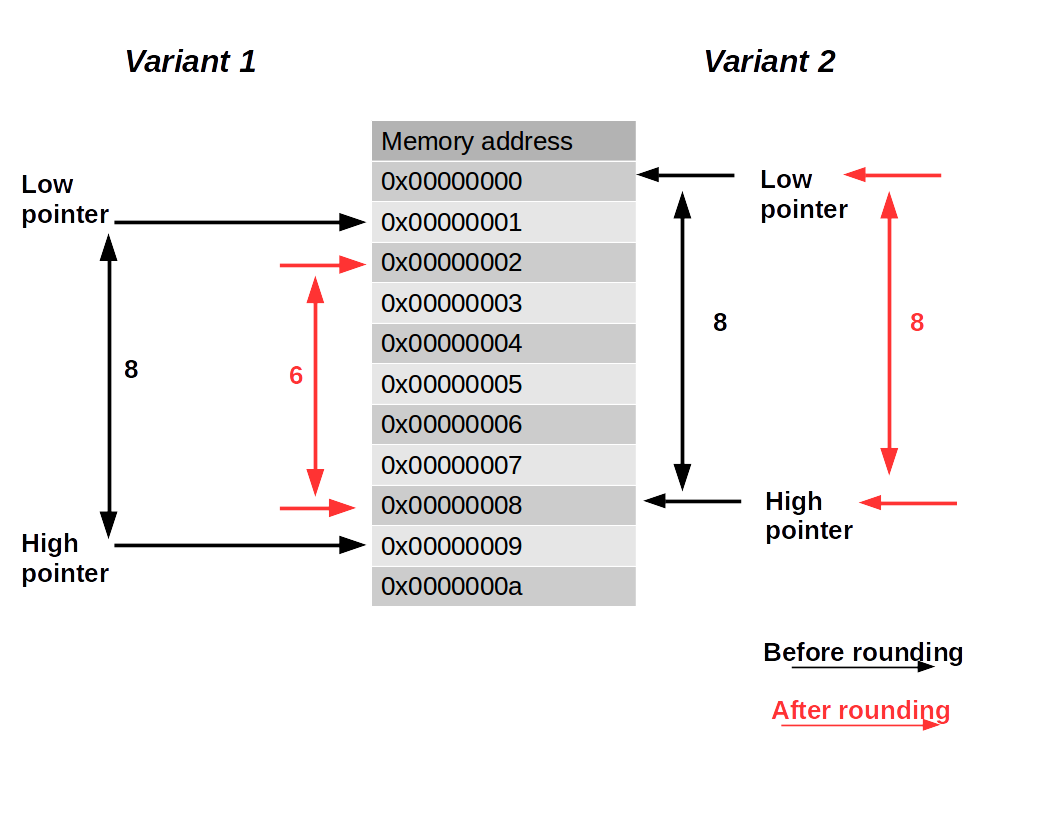
\includegraphics[width=0.65\textwidth]{RoundUpMemory}}
 \caption{Rounding to 2 in diverse variants}
 \label{fig:rounding}
\end{figure}
>>>>>>> 7fa6a02c7a9cf8e9d5fddf8d1e0dad030d78268a


\section{Writing a pointer or a padded structure}

Writing a pointer is also a big issue since the pointers will always be different among the variants.
Usually, writing those pointer values in a file or in a standard output is useless and thus, one could think that this problem won't occur in
real life programs. Nevertheless, we found a few out the the libx11 library does it with some pointers to GUI 
(Graphical User Interface) handler functions. These pointers are stored in a display buffer that is later on given to another thread 
thourgh a \texttt{writev()} system call.
Because of the important use of the Xlibraries, a lot of programs failed in the MVEE because of such problems.
\\ \\
In the same X libraries, threads exchange some specific structures. For performance reasons, the threads directly write the whole 
structure in a pipe by casting the struct pointer to character pointer. The other thread just casts it back when it receives it.
The problem here is that C compilers add some padding bytes to the structure. Once again, these padding bytes are introduced for performance
reasons (the processor is faster if the data are 4 bytes aligned). Technically, the compiler just ``jumps'' a few bytes to align 
the structure members. These jumped bytes being uninitialized, divergence is created as explained in \ref{uninit}. \\

\begin{lstlisting}[frame=single, caption=Writing a padded structure, label=lst:padstruct, language=C]
struct padded_struct {
    char ch1; // 1 byte
	      // 3 padding bytes
    int i1;   // 4 bytes on 64bits system
    int i2;   // 4 bytes
};

int main(int argc, char *argv[]) {
    struct padded_struct foo;
    
    foo.ch1 = 'a';
    foo.i1 = 0;
    foo.i2 = 1;
    
    printf("sizeof padded_struct is %ld\n", sizeof(foo)); 
      /* sizeof padded_struct is 12 */
    
    write(2, &foo, sizeof(foo));
      /* Argument mismatch triggered if ASLR is enabled */
    return 0;
}
\end{lstlisting}

=======
the structure members. These jumped bytes being uninitialized, divergence is created as explained in \ref{uninit}. See appendix \ref{padded} for the creation of a padded structure.
\\ \\ \\
>>>>>>> 7fa6a02c7a9cf8e9d5fddf8d1e0dad030d78268a

After having covered most of the address sensitive behaviors, we focused on finding either a general solution to fix these 
problems or a tool that would help the developer making his code MVEE compatible.
It appeared that the pointer to integer casts are the most common cause of address sensitivity and we then decided to focus on this 
problem.

\chapter{Tool development}

As the second part of our internship, my colleague and I built up a few tools that helped studying, detecting and solving address
sensitivity issues. This work also lead to the writing of a technical report for the laboratory.

\section{The delta strategy}

After a lot of brainstorming, we came with an idea that we later called the delta strategy.
The idea is to detect every pointer to integer cast and then apply some transformation on the integer so as to get the same value
in every variant. \\
In GHUMVEE, there is a constant offset between each variants' memory addresses. Thus, it is pretty easy to consider that one
variant is the master and that each ``slave'' has to know the offset between its memory layout and the master's.
The slaves would just have to add this delta to the freshly cast integer. \\ 
\image{label}{Delta strategy}{height=8cm}{delta_strategy.jpg} \\
But this strategy raises a new question: How to deal with cast backs (int->ptr->int)? \\ First, we spent a lot of time determining wether the program
genreal behavior would be alterated by this strategy in case of a cast back (integer to pointer). If some non linear computations
are applied to the integer, the result of the cast back value would be very different from what it should be without the delta 
strategy. But after studying it, it appears that every non linear operation on a memory address results in a totally unpredictable
value. Thus, the programmer wouldn't rely on this new pointer. So we could consider substracting the delta when a cast back is done. \\
But since the MVEE is a security software, we had to also study if this feature would create a security breach... And it does if casting
back is allowed. \\ The attacker would be able to overwite the integer (i.e. the cast pointer) with some malicious address, of course
this address only redirects to some malicious code in one variant. But if a cast back is done, every slave will substract its delta
value and the pointer will point to malicious in every single variant. \\ 
\image{delta_attack}{Attacking the delta strategy if the cast back is allowed}{height=8cm}{attacking_delta.jpg} \\

\section{Abstraction and cast back occurence analysis}

The idea behing the delta strategy is the creation of a ``virtual'' memory that is shared between the variants. \\
This can be generalized to every technique trying to inject a common integer value after a cast and we now know that we can't allow
cast back for security reasons. \\ Before totally giving up on this idea, we wanted to know how often such pointer to integer cast are
done. After all, if these are rare, it would still be possible to implement the delta strategy by slighlty modifying the original 
program. We also had the belief that integer to pointer casts are rare.\\ 
To do so, we decided to create our own clang plugin. Clang is a compiler which is part of the LLVM project. The LLVM project as 
the advantage of being pretty well documented and we already knew that creating a cast detection tool was highly doable. \\
Still, learning how to set up and use LLVM required a lot of effort. \\
After a few days, we had a generic clang plugin that was capable of detecting any kind of cast. During the rest of the internship,
we kept adding some features and modifications to this tool to make it more versatile ( error output, source file and line number of 
the cast, syntax tree dump...). \\ \\
Unfortunately, after running our tool on the most common C libraries, it appeared that a lost of integer to pointer cast were done.
The delta strategy couldn't be applied that way, it required at least some relaxation.

\section{Taint checking}

As to relax the whole idea of the delta strategy, we thought about not applying it to every cast. \\
We first wanted to apply it to every cast while giving the opportunity to the developper to manually disable it. But we could also do
it the other way round. We were not sure which solution would be the best since we didn't know if the cast which proportion of the 
could required the delta strategy. \\ Anyway, doing any of this solution and making the program crash until the programmer finds all
of the cast was not satisfactory.
We wanted a tool that could detect wether or not a cast was causing addressing sensitivity. We found out that a cast pointer was
address sensitive only if a variable affected by this cast was used in a condition or as an index.
Our idea was then to somehow mark the cast pointer and every single variable that was derivating from it and then check if the variables
used in conditions or index were marked. If such a marked variable was identified, we would just have to trace back to the origin of
the mark and notify it as address sensitive. \\ 
After discussing with a doctor, we discovered that this method is called taint checking \cite{taint}. \\
Taint checkers are known to highly slow down the program but it wasn't such a problem for us since we just needed it to prepare and 
adapt the program (the tool would only be used once to determine the address sensitive casts). The biggest problem was to find a good 
taint checker. Implementing one was not an option since it is very complicated and time consuming. On the other hand, most taint 
checkers were developed for a specific use and didn't fit our needs. We finally found out the valgrind's taint checker (taintgrind)
allowed the user to manually taint its sources. Of course, manually tainting the source was not an option. But this is where our
clang plugin came in handy: We could compile our programs and notify every single cast, we would then just have to create a script 
that would do some source to source compilation to add the tainting.
\\ 
Taintgrind outputing every single tainted instruction, we also had to write a script that detects the sink (a tainted variable used
in a condition or as an index) and traces back to the evil pointer cast. \\ \\
The source to source compilation was quite successful but still, some slighlty unusual syntax would imply some manual fix to have the
program running. Still, we tested the script on a few libraries just as a proof of concept and we didn't find any flaw in the taint
checking process. \\ \\
Still, the tool couldn't be seriously used and a form of delta strategy had to be implemented. \\

\section{Function inserting tool}

As my colleague was written a second report about the taint checking and delta strategy combination, I decided to develop another 
LLVM tool. Once again, going through the LLVM documentation was challenging but in the end, I managed to write a new tool that could
insert any function before any kind of cast or any other kind of instruction. \\ 
The tool uses LLVM's intermediate representation to detect the cast and grab the cast value. Then, the tools inserts the function we
want right before the cast. Of course, this function has to be compiled to the LLVM IR and linked to the main program we want to
work on.
This tool could now both apply the taint checking process and the last implementation of delta strategy we came up with.
Stijn Volckaert, the developer of GHUMVEE advised us to normalize the pointers after a cast. \\ \\
In the virtual memory model, the first bytes of a pointer are the memory page number of the data and the last bytes are the offset
to access the data. In GHUMVEE, the same pointer will only differ by the page number among the different variants, the offset 
being the same. \\ So the last idea we came with was just to change the page number of a pointer when it is cast to an integer.
The new page number being simply the order of the cast (value 1 assigned to the first pointer being cast, then 2,...).
A table has to be created to remember if a pointer has already been assigned a integer value.
By that mean, every cast pointer would have the same value. Plus, this implementation doesn't require any kind of communication between
the variants which is easier to implement and safer.\\
\image{stijn}{Normilizing pointers during pointer to integer cast}{height=8cm}{stijnsolution.jpg} \\

\chapter{Planning of the internship}


\begin{tableau}{planning}{Internship Planning}{|c|C{12cm}|}
    \hline
    June 6 to June 20 & Setting up GHUMVEE, reading papers about MVEE and code injection attacks. Minor GHUMVEE bug fixes.\\
    \hline
    June 21 to July 5 & Investigation on address sensitivity. implementation of a few IOCTLs in GHUMVEE. \\
    \hline
    July 6 to July 12 & Writing of the technical report for the DARPA.  \\
    \hline
    July 13 to August 2 &  Analysis of common hash tables to find a common pattern. Modelisation of the delta strategy.
implementation  the cast detection tool in LLVM. \\
    \hline
    August 3 to August 16 & Research on taint analysis. Implentation of a source to source compilation script to implement the taint.
implementation of a script to extract information from taintgrind's output.\\
    \hline
    August 16 to August 28 & Development of a new LLVM tool that inserts function after pointer casts. Mathematical formulation of the
taint checking model in MVEE. Writing of a internal technical report concerning all research from July 13 until the end of the internship.\\
    \hline
\end{tableau}


\partb{Conclusion}
Bla bla bla bla bla bla bla bla bla bla bla bla bla bla bla bla bla bla bla bla bla bla bla bla bla bla bla bla bla bla bla bla bla bla bla bla bla bla bla bla bla bla bla bla bla bla bla bla bla bla bla bla bla bla bla bla bla bla bla bla bla bla bla bla bla bla bla bla bla bla bla bla bla bla bla bla bla bla bla bla bla bla bla bla bla bla bla bla bla bla bla bla bla bla bla bla bla bla bla bla bla bla bla bla bla bla bla bla bla bla bla bla bla bla bla bla bla bla bla bla bla bla bla bla bla bla bla bla bla bla bla bla bla bla bla bla bla bla bla bla bla bla bla bla bla bla bla bla bla bla bla bla bla bla bla bla bla bla bla bla bla bla bla bla bla bla bla bla bla bla bla bla bla bla bla bla bla bla bla bla bla bla bla bla bla bla bla bla bla bla bla bla bla bla bla bla bla bla bla bla bla bla bla bla bla bla bla bla bla bla bla bla bla bla bla bla bla bla bla bla bla bla bla bla bla bla bla bla bla bla bla bla bla bla bla bla bla bla bla bla bla bla bla bla bla bla bla bla bla bla bla bla bla bla bla bla bla bla bla bla bla bla bla bla bla bla bla bla bla bla bla bla bla bla bla bla bla bla bla bla bla bla bla bla bla bla bla bla bla bla bla bla bla bla bla bla bla bla bla 



\afficheGlossaire

\afficheIndex

\listedestables

\listedesfigures



\bibliographystyle{plain}
\bibliography{biblio}


\partb{Appendix}

\begin{lstlisting}[frame=single, caption=Writing a padded structure, label=lst:padstruct, language=C]
struct padded_struct {
    char ch1; // 1 byte
	      // 3 padding bytes
    int i1;   // 4 bytes on 64bits system
    int i2;   // 4 bytes
};

int main(int argc, char *argv[]) {
    struct padded_struct foo;
    
    foo.ch1 = 'a';
    foo.i1 = 0;
    foo.i2 = 1;
    
    printf("sizeof padded_struct is %ld\n", sizeof(foo)); 
      /* sizeof padded_struct is 12 */
    
    write(2, &foo, sizeof(foo));
      /* Argument mismatch triggered if ASLR is enabled */
    return 0;
}
\end{lstlisting}\label{padded}

\end{document}